\documentclass[10pt,aspectratio=169]{beamer}

\usepackage{FiraSans}
\usepackage[T1]{fontenc}
\usepackage[utf8]{inputenc}
\usetheme{metropolis}

\usepackage{amsmath}
\def\mathfamilydefault{Latin Modern Math}

% Tikz
\usepackage{xcolor}
\usetikzlibrary{calc}
\usetikzlibrary{overlay-beamer-styles}
\usetikzlibrary{positioning}

\title{How JPEG works}
\date{February 9, 2021}
\author{Krzysztof Antoniak}

\begin{document}
\maketitle

\begin{frame}[plain]{JPEG standard}
	\begin{itemize}
		\item Created by Joint Photographic Experts Group in 1992
		\item Lossy compression of images with controllable quality settings
		\begin{itemize}
			\item Lossy - does not work for medical imaging etc.
			\item Designed for photos, won't work for illustrations or text
		\end{itemize}
		\item Probably the most popular format for photos
		\begin{itemize}
			\item Superseded by JPEG 2000, which didn't become as popular
		\end{itemize}
		\item There are lots of options and extensions, we will look at the simplest case
	\end{itemize}
\end{frame}

\begin{frame}[c,plain]
	\vspace{5pt}
	\begin{figure}
		\centering
		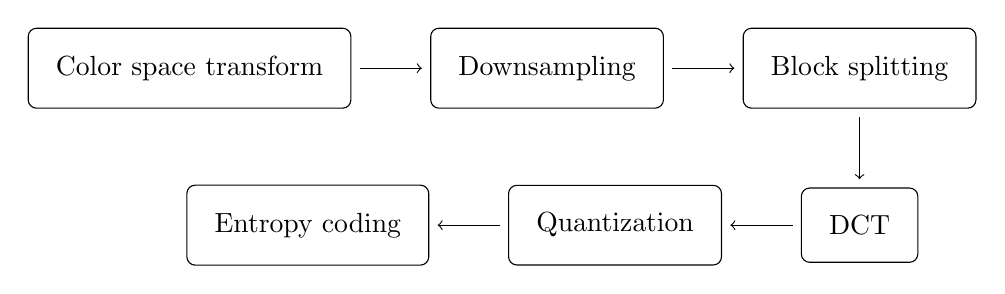
\begin{tikzpicture}
			\node[draw,rounded corners=3pt,inner sep=10pt] (a) {Color space transform};
			\node[draw,rounded corners=3pt,inner sep=10pt,right=of a] (b) {Downsampling};
			\node[draw,rounded corners=3pt,inner sep=10pt,right=of b] (c) {Block splitting};
			\node[draw,rounded corners=3pt,inner sep=10pt,below=of c] (d) {DCT};
			\node[draw,rounded corners=3pt,inner sep=10pt,left=of d] (e) {Quantization};
			\node[draw,rounded corners=3pt,inner sep=10pt,left=of e] (f) {Entropy coding};
			
			\draw[->, shorten >=3pt, shorten <=3pt] (a) -- (b);
			\draw[->, shorten >=3pt, shorten <=3pt] (b) -- (c);
			\draw[->, shorten >=3pt, shorten <=3pt] (c) -- (d);
			\draw[->, shorten >=3pt, shorten <=3pt] (d) -- (e);
			\draw[->, shorten >=3pt, shorten <=3pt] (e) -- (f);
		\end{tikzpicture}
		\vspace{10pt}
		\caption{Steps of JPEG compression.}
	\end{figure}
\end{frame}

\begin{frame}[c,plain]
	\vspace{12pt}
	\begin{figure}
		\centering
		\includegraphics[height=0.5\textwidth]{images/mimuw.jpg}
		\caption{Source photo (CC BY-SA 3.0 Krzysztof Dudzik \cite{wiki:mimuw})}
	\end{figure}
\end{frame}

\begin{frame}[c,plain]
	\vspace{12pt}
	\begin{figure}
		\centering
		\includegraphics[height=0.5\textwidth]{images/mimuw-square-128-upscaled.png}
		\caption{Test image before compression, 128$\times$128 pixels.}
	\end{figure}
\end{frame}

\section{Color spaces}

\begin{frame}[plain]{Color perception}
	\begin{itemize}
		\item Human eye consists of millions of "light sensors": rods and cones
		\item Cones allow reception of color
		\begin{itemize}
			\item Cones respond to light wavelengths corresponding with red, green and blue colors
			\item They are placed in the central part of the eye
		\end{itemize}
		\item Rods are sensitive to light intensity
		\begin{itemize}
			\item Rods allow us to operate in low light
			\item In some areas of FOV we can recognize shapes but no colors
		\end{itemize}
	\end{itemize}
\end{frame}

\begin{frame}[plain]{Displaying colors - RGB space}
	\begin{itemize}
		\item Machines operate differently than humans
		\item Each pixel of the monitor emits light, which is a combination of tiny red, green and blue diodes
		\begin{itemize}
			\item Amount of light determines brightness
			\item Mixing proportions generates hue
		\end{itemize}
		\item This leads to analyzing (and storing) colors in terms of color channels
		\begin{itemize}
			\item For each pixel there are three components: R, G, and B
			\item Normalized values are stored as numbers between $0$ and $2^b$
			\item Often $b=8$, and we get a total of $ \left(2^8\right)^3 > 16 000 000 $ colors
		\end{itemize}
		\item It's convenient for computers but far from how out visual system works
	\end{itemize}
\end{frame}

\begin{frame}[c,plain]
\vspace{5pt}
\begin{figure}
	\centering
	\begin{tikzpicture}
		\fill[white, fill opacity=0] (-2,1) rectangle (9,0);
		
		\node (rgb) at (3.5, 3.8) {\includegraphics[height=0.2\textwidth]{images/mimuw-square-128-upscaled.png}};
		\node (red) at (0,0) {\includegraphics[height=0.2\textwidth]{images/mimuw-square-128-rgb-red-upscaled.png}};
		\node (green) at (3.5,0) {\includegraphics[height=0.2\textwidth]{images/mimuw-square-128-rgb-green-upscaled.png}};
		\node (blue) at (7,0) {\includegraphics[height=0.2\textwidth]{images/mimuw-square-128-rgb-blue-upscaled.png}};
		
		\node[below] at (red.south) {\textsc{r}};
		\node[below] at (green.south) {\textsc{g}};
		\node[below] at (blue.south) {\textsc{b}};
		
		\draw [<-, shorten >=3pt, shorten <=3pt] (red) -- (rgb);
		\draw [<-, shorten >=3pt, shorten <=3pt] (green) -- (rgb);
		\draw [<-, shorten >=3pt, shorten <=3pt] (blue) -- (rgb);
		
		% Annotations			
		\pause
		
		\definecolor{mygreen}{rgb}{0,0.8,0}
		\definecolor{myblue}{rgb}{0.2,0.2,1}
		
		\draw[myblue,thick] ($ (rgb) + (1.11,1.08) $) circle (0.3);
		\draw[myblue,thick] ($ (blue) + (1.11,1.08) $) circle (0.3);
		
		\draw[mygreen,thick,rounded corners] ($ (rgb) + (-0.6,-0.8) $) rectangle ($ (rgb) + (1.5,-1.5) $);
		\draw[mygreen,thick,rounded corners] ($ (green) + (-0.6,-0.8) $) rectangle ($ (green) + (1.5,-1.5) $);
		
		\node[align=left] at (7.3,3.8) {
			\footnotesize Channel pixel has greater \\
			\footnotesize value if source image pixel \\
			\footnotesize matches channel color.};
	\end{tikzpicture}
	\caption{Test image decomposed into RGB channels.}
\end{figure}
\end{frame}

\begin{frame}[plain]{An alternative - YCbCr}
	\begin{itemize}
		\item There are multiple ways of storing color information
		\item Compression algorithms use the fact that we are much more sensitive to brightness than colors
		\item YCbCr is the defacto standard in many multimedia applications
		\item It has 3 color channels:
		\begin{itemize}
			\item Y, luma - color brightness
			\item Cb - blueness
			\item Cr - redness
		\end{itemize}
		\item All colors (including green) can be derived from this information
		\item This is much closer to how human eye works
		\begin{itemize}
			\item We can discard some information from less important channels
			\item Optional downsampling lowers resolution of channels
		\end{itemize}
	\end{itemize}
\end{frame}

\begin{frame}[c,plain]
	\vspace{5pt}
	\begin{figure}
		\centering
		\begin{tikzpicture}
			\node (ycbcr) at (3.5, 3.8) {\includegraphics[height=0.2\textwidth]{images/mimuw-square-128-upscaled.png}};
			\node (luma) at (0,0) {\includegraphics[height=0.2\textwidth]{images/mimuw-square-128-ycbcr-luma-upscaled.png}};
			\node (blueness) at (3.5,0) {\includegraphics[height=0.2\textwidth]{images/mimuw-square-128-ycbcr-blueness-upscaled.png}};
			\node (redness) at (7,0) {\includegraphics[height=0.2\textwidth]{images/mimuw-square-128-ycbcr-redness-upscaled.png}};
			
			\node[below] at (luma.south) {\textsc{\small Luma}};
			\node[below] at (blueness.south) {\textsc{\small Blueness}};
			\node[below] at (redness.south) {\textsc{\small Redness}};
			
			\draw [<-, shorten >=3pt, shorten <=3pt] (luma) -- (ycbcr);
			\draw [<-, shorten >=3pt, shorten <=3pt] (blueness) -- (ycbcr);
			\draw [<-, shorten >=3pt, shorten <=3pt] (redness) -- (ycbcr);
		\end{tikzpicture}
		\caption{Test image decomposed into YCbCr channels.}
	\end{figure}
\end{frame}

\section{DCT}

\begin{frame}{Discrete Cosine Transform (DCT)}
	\metroset{block=fill}
	\begin{block}{Discrete Cosine Transform Matrix}
		\vspace{0.5em}
		\begin{equation*}
			C_{i,j} =
				\begin{cases}
					\sqrt{\frac{1}{N}} \cos{\frac{(2j+1)i\pi}{2N}}  & i=0, \\
					\sqrt{\frac{2}{N}} \cos{\frac{(2j+1)i\pi}{2N}}  & i>0
				\end{cases}
		\end{equation*}
	\end{block}
	\begin{itemize}
		\item Each row contains cosine values
		\item Row values are sampled with increasing frequency
		\item Outer product of rows generates a basis for $ \mathbb{R}^{N \times N} $
		\item This is an orthonormal basis $\Rightarrow C_{i,j}' = C_{j,i}$ 
	\end{itemize}
\end{frame}

\begin{frame}[c,plain]
	\begin{figure}
		\centering
		\includegraphics[height=0.5\textwidth]{images/dct-basis.png}
		\caption{DCT basis matrices for 8$\times$8 block.}
	\end{figure}
\end{frame}

\begin{frame}{Applying DCT}
	\begin{enumerate}
		\item Take 8$\times$8 block $B$ of channel values between $0$ --- $256$.
		\item Subtract $128$ to center around $0$.
		\item Compute $ C \cdot B \cdot C' $.
	\end{enumerate}
\end{frame}

%step
\newcommand{\datablock}[2]{
	\begin{scope}[scale=#1/8]
		\path[fill=white] (0,0) rectangle (8,8);
		\foreach \x[
			evaluate=\x as \startx using {\x}] in {0,...,7}{
			\foreach \y[
				evaluate=\y as \i using int(8*\y+\x),
				evaluate=\y as \value using {int(#2[\i])},
				evaluate=\y as \starty using {-\y + 8}] in {0,...,7}{
				\node at ($(\startx, \starty) + (0.5,-0.5) $) {\tiny \value};
			}
		}
		\draw [draw=black!20!white] (0,0) grid (8,8) rectangle (0,0);
	\end{scope}
}

\def\sampleBlockLuma{{
	124,  159,  118,  121,  115,  176,  174,  125,
	126,  161,  118,  120,  114,  175,  174,  124,
	130,  161,  115,  118,  110,  176,  173,  123,
	129,  164,  113,  116,  105,  176,  174,  123,
	127,  139,  114,  117,  102,  177,  175,  124,
	129,  117,  117,  119,   99,  175,  174,  126,
	129,  123,  114,  113,   94,  175,  174,  126,
	127,  120,  122,  120,   88,  175,  173,  127,
}}

\def\sampleBlockLumaShifted{{
	-4,  31, -10,  -7, -13,  48,  46,  -3,
	-2,  33, -10,  -8, -14,  47,  46,  -4,
	2,  33, -13, -10, -18,  48,  45,  -5,
	1,  36, -15, -12, -23,  48,  46,  -5,
	-1,  11, -14, -11, -26,  49,  47,  -4,
	1, -11, -11,  -9, -29,  47,  46,  -2,
	1,  -5, -14, -15, -34,  47,  46,  -2,
	-1,  -8,  -6,  -8, -40,  47,  45,  -1
}}

\def\sampleBlockDctCoeffs{{
	60,  -75,   53,   81, -134,   45,  -15,  -64,
	25,   18,   -6,    3,   -9,  -33,  -29,   -3,
	-2,   -4,   -3,   -6,    2,    6,    7,    2,
	-4,   -9,   -5,    2,    6,    6,    6,    5,
	2,    2,    1,   -2,   -4,   -2,   -2,   -4,
	-0,    2,    4,    3,   -2,   -5,   -4,   -2,
	-0,   -2,   -3,   -2,    3,    5,    5,    1,
	-1,   -1,    1,    2,   -0,   -0,    0,    0
}}

\def\QTzero{{
	16, 11, 12, 14, 12,  10, 16, 14,
	13, 14, 18, 17, 16,  19, 24, 40,
	26, 24, 22, 22, 24,  49, 35, 37,
	29, 40, 58, 51, 61,  60, 57, 51,
	56, 55, 64, 72, 92,  78, 64, 68,
	87, 69, 55, 56, 80, 109, 81, 87,
 	95, 98, 103, 104, 103, 62, 77, 113,
	121, 112, 100, 120, 92, 101, 103, 99
}}

\def\sampleBlockQuantCoeffs{{
	4, -7, 4, 6, -11, 5, -1, -5,
	2, 1, 0, 0, -1, -2, -1, 0,
	0, 0, 0, 0, 0, 0, 0, 0,
	0, 0, 0, 0, 0, 0, 0, 0,
	0, 0, 0, 0, 0, 0, 0, 0,
	0, 0, 0, 0, 0, 0, 0, 0,
	0, 0, 0, 0, 0, 0, 0, 0,
	0, 0, 0, 0, 0, 0, 0, 0,
}}

\def\sampleBlockDequantCoeffs{{
	64, -77, 48, 84, -132, 50, -16, -70,
	26, 14, 0, 0, -16, -38, -24, 0,
	0, 0, 0, 0, 0, 0, 0, 0,
	0, 0, 0, 0, 0, 0, 0, 0,
	0, 0, 0, 0, 0, 0, 0, 0,
	0, 0, 0, 0, 0, 0, 0, 0,
	0, 0, 0, 0, 0, 0, 0, 0,
	0, 0, 0, 0, 0, 0, 0, 0,
}}

\def\sampleBlockDedctCoeffs{{
	-3, 39, -10, -10, -13, 51, 47, -2,
	-2, 35, -10, -9, -14, 51, 47, -2,
	-2, 28, -11, -8, -18, 50, 47, -3,
	-1, 19, -12, -7, -22, 50, 47, -3,
	0, 9, -12, -6, -26, 49, 46, -3,
	1, 0, -13, -5, -30, 48, 46, -4,
	2, -7, -14, -4, -33, 48, 46, -4,
	2, -10, -14, -4, -35, 48, 46, -5,
}}

\def\sampleBlockUnshiftedLuma{{
	125, 167, 118, 118, 115, 179, 175, 126,
	126, 163, 118, 119, 114, 179, 175, 126,
	126, 156, 117, 120, 110, 178, 175, 125,
	127, 147, 116, 121, 106, 178, 175, 125,
	128, 137, 116, 122, 102, 177, 174, 125,
	129, 128, 115, 123, 98, 176, 174, 124,
	130, 121, 114, 124, 95, 176, 174, 124,
	130, 118, 114, 124, 93, 176, 174, 123,
}}

\begin{frame}[c,plain]
	\vspace{5pt}
	\begin{figure}
		\centering
		\begin{tikzpicture}
			\fill[white, fill opacity=0] (-5,1) rectangle (5,0);
			\node[inner sep=0pt] (rgb) at (0, 0) {\includegraphics[height=0.4\textwidth]{images/mimuw-square-128-upscaled.png}};
			\node[above=5pt,visible on=<1>] at (rgb.north) {\textsc{\small Base image}};
			\node[above=5pt,visible on=<2->] at (rgb.north) {\textsc{\small Blocks}};
			
			\pause
			\begin{scope}[scale=5.6/16]
				\foreach \x in {0,...,15}{
					\foreach \y[
					evaluate=\x as \m using {Mod(\x,2)}] in {0,2,4,6,8,10,12,14}{
						\draw [draw=none,fill=black,fill opacity=0.4] ($ (rgb.south west) + (\x,\y+\m) $) rectangle ($ (rgb.south west) + (\x,\y+\m) + (1,1) $);
					}
				}
			\end{scope}
			
			\pause
			\begin{scope}[scale=5.6/16,shift={(rgb.south west)}]
				\draw[draw=none,fill=black!5!white] (8,4) -- (7,4) -- (7,5) -- (10,15) -- (10,7) -- (18,7) -- cycle;
				\draw[draw=none,fill=black!8!white] (8,4) -- (7,4) -- (10,7) -- (18,7) -- cycle;
				\node[inner sep=0pt] at (14,11) {\includegraphics[height=80pt]{images/dct-block-rgb-upscaled.png}};
			\end{scope}
		\end{tikzpicture}
		\caption{Splitting image into blocks.}
	\end{figure}
\end{frame}

\begin{frame}[c,plain]
	\vspace{5pt}
	\begin{figure}
		\centering
		\begin{tikzpicture}
			\node (rgb) at (0, 0) {\includegraphics[height=0.18\textwidth]{images/dct-block-rgb-upscaled.png}};
			\node (luma) at (3.6, -1.5) {\includegraphics[height=0.18\textwidth]{images/dct-block-luma-upscaled.png}};
			\node (coeffs) at (10.8, -1.5) {\includegraphics[height=0.18\textwidth]{images/dct-block-coeffs-upscaled.png}};
			
			\node (lumaData) at (3.6,1.5){\tikz{\datablock{2.52}{\sampleBlockLuma}}};
			\node (shiftData) at (7.2,0){\tikz{\datablock{2.52}{\sampleBlockLumaShifted}}};
			\node (coeffsData) at (10.8,1.5){\tikz{\datablock{2.52}{\sampleBlockDctCoeffs}}};
			
			\node[above] at (rgb.north) {\textsc{\small RGB}};
			\node[above] at (lumaData.north) {\textsc{\small Luma}};
			\node[above] at (shiftData.north) {\textsc{\small Shifted luma}};
			\node[above] at (coeffsData.north) {\textsc{\small DCT Coefficients}};
			
			\coordinate (lumaMid) at ($(lumaData)!0.5!(luma)$);
			\coordinate (coeffsMid) at ($(coeffs)!0.5!(coeffsData)$);
			\draw [->, shorten >=42pt, shorten <=2pt] (rgb) -- node [midway,above,align=center,xshift=-20pt] {1} (lumaMid);
			\draw [->, shorten <=42pt] (lumaMid) -- node [midway,above,align=center,xshift=21pt] {2} (shiftData);
			\draw [->, shorten >=42pt] (shiftData) -- node [midway,above,align=center,xshift=-21pt] {3} (coeffsMid);
			
		\end{tikzpicture}
		\caption{Applying transform step to a single luma block. (All values rounded).}
	\end{figure}
\end{frame}

\begin{frame}[c,plain]
	\vspace{5pt}
	\begin{figure}
		\centering
		\begin{tikzpicture}
			\node (rgb) at (0, 0) {\includegraphics[height=0.28\textwidth]{images/mimuw-square-128-upscaled.png}};
			\node (coeffs) at (4.8, 0) {\includegraphics[height=0.28\textwidth]{images/mimuw-square-128-coeffs-upscaled.png}};
			\node (basis) at (9.6, 0) {\includegraphics[height=0.28\textwidth]{images/dct-basis.png}};
			
			\node[above] at (rgb.north) {\textsc{\small Base image}};
			\node[above] at (coeffs.north) {\textsc{\small DCT coefficients}};
			\node[above] at (basis.north) {\textsc{\small DCT basis}};
			
			\pause
			\node[above] (noteSky) at ($ (coeffs.north west) + (-0.5,0.6) $) {\footnotesize Almost uniform sky};
			\coordinate (pointSky) at ($ (coeffs) + (-1.75,1.75) $);
			\draw[thick,->] (noteSky) to [out=-70,in=150] (pointSky);
			
			\pause
			\node[above] (noteVert) at ($ (coeffs.south west) + (-0.25,-0.8) $) {\footnotesize Vertical columns};
			\coordinate (pointVert) at ($ (coeffs) + (-0.5,-1) $);
			\draw[thick,->] (noteVert) to [out=70,in=180] (pointVert);
			
			\pause
			\node[above] (noteHor) at ($ (coeffs.south east) + (0.25,-0.8) $) {\footnotesize Horizontal part};
			\coordinate (pointHor) at ($ (coeffs) + (1.5,-1.5) $);
			\draw[thick,->] (noteHor) to [out=100,in=-10] (pointHor);
			
		\end{tikzpicture}
		\caption{Transform applied to all luma blocks.}
	\end{figure}
\end{frame}

\begin{frame}{Quantization}
	\begin{itemize}
		\item Humans often miss small frequency changes
		\begin{itemize}
			\item We care less about more detailed basis elements
			\item Dropping then leaves more space for more important information
		\end{itemize}
		\item JPEG compression scales DCT coefficients
		\begin{itemize}
			\item Values get small and rounded, we lose some information
			\item Scaling is not uniform - that's the lossy part
			\item The bigger the coefficient, the more information we lose with rounding
		\end{itemize}
		\item Coefficients are tuned for psychovisual quality
		\begin{itemize}
			\item JPEG provides sample quantization tables
			\item There are different tables for different quality settings
			\item Software often provides custom tables, embedded with the file
		\end{itemize}
	\end{itemize}
\end{frame}

\begin{frame}[c,plain]
\vspace{5pt}
\begin{figure}
	\centering
	\vspace{5pt}
	\begin{tikzpicture}
		\path[fill=white,fill on=<1>] (0,0) rectangle (6.4,6.4);
		\foreach \x[
			evaluate=\x as \startx using {\x*.8}] in {0,...,7}{
			\foreach \y[
				evaluate=\y as \i using int(\y*8+\x),
				evaluate=\y as \value using {\QTzero[\i]},
				evaluate=\y as \starty using {-\y*.8 + 6.4},
				evaluate=\y as \strength using {100*\value/128},
				evaluate=\y as \textcolor using \strength<50?100:0] in {0,...,7}{
				\path[fill=black!\strength!white,fill on=<2->] ($(\startx, \starty)$) rectangle ($(\startx, \starty) + .8*(1,-1) $);
				\node[text=black!\textcolor!white,text on=<2->] at ($(\startx, \starty) + (0.4,-0.4) $) {\value};
			}
		}
		\draw [draw=black!40!white, xstep=.8, ystep=.8] (0,0) grid (6.4,6.4) rectangle (0,0);
	\end{tikzpicture}
	\caption{Sample quantization table for luma component (GIMP, q=50).}
\end{figure}
\end{frame}

\begin{frame}[c,plain]
	\vspace{5pt}
	\begin{figure}
		\centering
		\vspace{5pt}
		\begin{tikzpicture}
			\path[fill=white] (0,0) rectangle (6.4,6.4);
			\foreach \x[
			evaluate=\x as \startx using {\x*.8}] in {0,...,7}{
				\foreach \y[
				evaluate=\y as \i using int(\y*8+\x),
				evaluate=\y as \value using {int(\sampleBlockDctCoeffs[\i])},
				evaluate=\y as \starty using {-\y*.8 + 6.4}] in {0,...,7}{
					\path[fill=white] ($(\startx, \starty)$) rectangle ($(\startx, \starty) + .8*(1,-1) $);
					\node at ($(\startx, \starty) + (0.4,-0.4) $) {\value};
				}
			}
			\draw [draw=black!40!white, xstep=.8, ystep=.8] (0,0) grid (6.4,6.4) rectangle (0,0);
		\end{tikzpicture}
		\caption{Sample block before quantization.}
	\end{figure}
\end{frame}

\begin{frame}[c,plain]
	\vspace{5pt}
	\begin{figure}
		\centering
		\vspace{5pt}
		\begin{tikzpicture}
			\path[fill=white] (0,0) rectangle (6.4,6.4);
			\foreach \x[
			evaluate=\x as \startx using {\x*.8}] in {0,...,7}{
				\foreach \y[
				evaluate=\y as \i using int(\y*8+\x),
				evaluate=\y as \value using {int(\sampleBlockQuantCoeffs[\i])},
				evaluate=\y as \starty using {-\y*.8 + 6.4},
				evaluate=\y as \strength using {\value==0?10:0}] in {0,...,7}{
					\path[fill=black!\strength!white,fill on=<2->] ($(\startx, \starty)$) rectangle ($(\startx, \starty) + .8*(1,-1) $);
					\node at ($(\startx, \starty) + (0.4,-0.4) $) {\value};
				}
			}
			\draw [draw=black!40!white, xstep=.8, ystep=.8] (0,0) grid (6.4,6.4) rectangle (0,0);
		\end{tikzpicture}
		\caption{Sample block after quantization.}
	\end{figure}
\end{frame}

\begin{frame}[standout]
	\vspace{5pt}
	How to decompress image? \\
	Run everything backwards!
\end{frame}

\begin{frame}[c,plain]
	\vspace{5pt}
	\begin{figure}
		\centering
		\vspace{5pt}
		\begin{tikzpicture}
			\path[fill=white] (0,0) rectangle (5.6,5.6);
			\foreach \x[
			evaluate=\x as \startx using {\x*.7}] in {0,...,7}{
				\foreach \y[
				evaluate=\y as \i using int(\y*8+\x),
				evaluate=\y as \value using {int(\sampleBlockDctCoeffs[\i])},
				evaluate=\y as \starty using {-\y*.7 + 5.6}] in {0,...,7}{
					\node at ($(\startx, \starty) + (0.35,-0.35) $) {\value};
				}
			}
			\draw [draw=black!40!white, xstep=.7, ystep=.7] (0,0) grid (5.6,5.6) rectangle (0,0);
			
			\path[fill=white] (6,0) rectangle (11.6,5.6);
			\foreach \x[
			evaluate=\x as \startx using {6+\x*.7}] in {0,...,7}{
				\foreach \y[
				evaluate=\y as \i using int(\y*8+\x),
				evaluate=\y as \value using {int(\sampleBlockDequantCoeffs[\i])},
				evaluate=\y as \starty using {-\y*.7 + 5.6}] in {0,...,7}{
					\node at ($(\startx, \starty) + (0.35,-0.35) $) {\value};
				}
			}
			\draw [draw=black!40!white, xstep=.7, ystep=.7, shift={(6,0)}] (0,0) grid (5.6,5.6) rectangle (0,0);
		\end{tikzpicture}
		\caption{DCT coefficients before and during decompression.}
	\end{figure}
\end{frame}

\begin{frame}[c,plain]
	\vspace{5pt}
	\begin{figure}
		\centering
		\vspace{5pt}
		\begin{tikzpicture}
			\node[inner sep=0pt] at (2.8,2.8) {\includegraphics[height=0.4\textwidth]{images/dct-block-coeffs-upscaled.png}};
			\node[inner sep=0pt] at (8.8,2.8) {\includegraphics[height=0.4\textwidth]{images/dct-block-decomp-coeffs-upscaled.png}};
		\end{tikzpicture}
		\caption{DCT coefficients before and during decompression (as image).}
	\end{figure}
\end{frame}

\begin{frame}[c,plain]
	\vspace{5pt}
	\begin{figure}
		\centering
		\vspace{5pt}
		\begin{tikzpicture}
			\path[fill=white] (0,0) rectangle (5.6,5.6);
			\foreach \x[
			evaluate=\x as \startx using {\x*.7}] in {0,...,7}{
				\foreach \y[
				evaluate=\y as \i using int(\y*8+\x),
				evaluate=\y as \value using {int(\sampleBlockLumaShifted[\i])},
				evaluate=\y as \starty using {-\y*.7 + 5.6}] in {0,...,7}{
					\node at ($(\startx, \starty) + (0.35,-0.35) $) {\value};
				}
			}
			\draw [draw=black!40!white, xstep=.7, ystep=.7] (0,0) grid (5.6,5.6) rectangle (0,0);
			
			\path[fill=white] (6,0) rectangle (11.6,5.6);
			\foreach \x[
			evaluate=\x as \startx using {6+\x*.7}] in {0,...,7}{
				\foreach \y[
				evaluate=\y as \i using int(\y*8+\x),
				evaluate=\y as \value using {int(\sampleBlockDedctCoeffs[\i])},
				evaluate=\y as \starty using {-\y*.7 + 5.6}] in {0,...,7}{
					\node at ($(\startx, \starty) + (0.35,-0.35) $) {\value};
				}
			}
			\draw [draw=black!40!white, xstep=.7, ystep=.7, shift={(6,0)}] (0,0) grid (5.6,5.6) rectangle (0,0);
		\end{tikzpicture}
		\caption{Shifted luma coefficients before and during decompression.}
	\end{figure}
\end{frame}

\begin{frame}[c,plain]
\vspace{5pt}
\begin{figure}
	\centering
	\vspace{5pt}
	\begin{tikzpicture}
		\path[fill=white] (0,0) rectangle (5.6,5.6);
		\foreach \x[
		evaluate=\x as \startx using {\x*.7}] in {0,...,7}{
			\foreach \y[
			evaluate=\y as \i using int(\y*8+\x),
			evaluate=\y as \value using {int(\sampleBlockLuma[\i])},
			evaluate=\y as \starty using {-\y*.7 + 5.6}] in {0,...,7}{
				\node at ($(\startx, \starty) + (0.35,-0.35) $) {\value};
			}
		}
		\draw [draw=black!40!white, xstep=.7, ystep=.7] (0,0) grid (5.6,5.6) rectangle (0,0);
		
		\path[fill=white] (6,0) rectangle (11.6,5.6);
		\foreach \x[
		evaluate=\x as \startx using {6+\x*.7}] in {0,...,7}{
			\foreach \y[
			evaluate=\y as \i using int(\y*8+\x),
			evaluate=\y as \value using {int(\sampleBlockUnshiftedLuma[\i])},
			evaluate=\y as \starty using {-\y*.7 + 5.6}] in {0,...,7}{
				\node at ($(\startx, \starty) + (0.35,-0.35) $) {\value};
			}
		}
		\draw [draw=black!40!white, xstep=.7, ystep=.7, shift={(6,0)}] (0,0) grid (5.6,5.6) rectangle (0,0);
	\end{tikzpicture}
	\caption{Luma coefficients before and during decompression.}
\end{figure}
\end{frame}

\begin{frame}[c,plain]
\vspace{5pt}
\begin{figure}
	\centering
	\vspace{5pt}
	\begin{tikzpicture}
		\node[inner sep=0pt] at (2.8,2.8) {\includegraphics[height=0.4\textwidth]{images/dct-block-luma-upscaled.png}};
		\node[inner sep=0pt] at (8.8,2.8) {\includegraphics[height=0.4\textwidth]{images/dct-block-decomp-luma-upscaled.png}};
	\end{tikzpicture}
	\caption{Luma coefficients before and during decompression (as image).}
\end{figure}
\end{frame}

\begin{frame}[c,plain]
	\vspace{5pt}
	\begin{figure}
		\centering
		\vspace{5pt}
		\begin{tikzpicture}
			\node (q0) at (0,0) {\includegraphics[height=0.22\textwidth]{images/mimuw-square-128-q0-upscaled.png}};
			\node (q25) at (3.4,0) {\includegraphics[height=0.22\textwidth]{images/mimuw-square-128-q25-upscaled.png}};
			\node (q50) at (6.8,0) {\includegraphics[height=0.22\textwidth]{images/mimuw-square-128-q50-upscaled.png}};
			\node (q75) at (10.2,0) {\includegraphics[height=0.22\textwidth]{images/mimuw-square-128-q75-upscaled.png}};
			
			\node[below] at (q0.south) {0};
			\node[below] at (q25.south) {25};
			\node[below] at (q50.south) {50};
			\node[below] at (q75.south) {75};
		\end{tikzpicture}
		\caption{Comparison of compression quality settings (as exported from GIMP).}
	\end{figure}
\end{frame}

\begin{frame}{References}
  \nocite{sayood2017introduction}
  \bibliography{refs}
  \bibliographystyle{abbrv}
\end{frame}

\end{document}